% Options for packages loaded elsewhere
\PassOptionsToPackage{unicode}{hyperref}
\PassOptionsToPackage{hyphens}{url}
%
\documentclass[
]{article}
\usepackage{lmodern}
\usepackage{amssymb,amsmath}
\usepackage{ifxetex,ifluatex}
\ifnum 0\ifxetex 1\fi\ifluatex 1\fi=0 % if pdftex
  \usepackage[T1]{fontenc}
  \usepackage[utf8]{inputenc}
  \usepackage{textcomp} % provide euro and other symbols
\else % if luatex or xetex
  \usepackage{unicode-math}
  \defaultfontfeatures{Scale=MatchLowercase}
  \defaultfontfeatures[\rmfamily]{Ligatures=TeX,Scale=1}
\fi
% Use upquote if available, for straight quotes in verbatim environments
\IfFileExists{upquote.sty}{\usepackage{upquote}}{}
\IfFileExists{microtype.sty}{% use microtype if available
  \usepackage[]{microtype}
  \UseMicrotypeSet[protrusion]{basicmath} % disable protrusion for tt fonts
}{}
\makeatletter
\@ifundefined{KOMAClassName}{% if non-KOMA class
  \IfFileExists{parskip.sty}{%
    \usepackage{parskip}
  }{% else
    \setlength{\parindent}{0pt}
    \setlength{\parskip}{6pt plus 2pt minus 1pt}}
}{% if KOMA class
  \KOMAoptions{parskip=half}}
\makeatother
\usepackage{xcolor}
\IfFileExists{xurl.sty}{\usepackage{xurl}}{} % add URL line breaks if available
\IfFileExists{bookmark.sty}{\usepackage{bookmark}}{\usepackage{hyperref}}
\hypersetup{
  pdftitle={Diabetes Data Diving Write-up},
  pdfauthor={Nilai Vemula, Anvitha Kosuraju, and Sithara Samudrala},
  hidelinks,
  pdfcreator={LaTeX via pandoc}}
\urlstyle{same} % disable monospaced font for URLs
\usepackage{color}
\usepackage{fancyvrb}
\newcommand{\VerbBar}{|}
\newcommand{\VERB}{\Verb[commandchars=\\\{\}]}
\DefineVerbatimEnvironment{Highlighting}{Verbatim}{commandchars=\\\{\}}
% Add ',fontsize=\small' for more characters per line
\newenvironment{Shaded}{}{}
\newcommand{\AlertTok}[1]{\textcolor[rgb]{1.00,0.00,0.00}{\textbf{#1}}}
\newcommand{\AnnotationTok}[1]{\textcolor[rgb]{0.38,0.63,0.69}{\textbf{\textit{#1}}}}
\newcommand{\AttributeTok}[1]{\textcolor[rgb]{0.49,0.56,0.16}{#1}}
\newcommand{\BaseNTok}[1]{\textcolor[rgb]{0.25,0.63,0.44}{#1}}
\newcommand{\BuiltInTok}[1]{#1}
\newcommand{\CharTok}[1]{\textcolor[rgb]{0.25,0.44,0.63}{#1}}
\newcommand{\CommentTok}[1]{\textcolor[rgb]{0.38,0.63,0.69}{\textit{#1}}}
\newcommand{\CommentVarTok}[1]{\textcolor[rgb]{0.38,0.63,0.69}{\textbf{\textit{#1}}}}
\newcommand{\ConstantTok}[1]{\textcolor[rgb]{0.53,0.00,0.00}{#1}}
\newcommand{\ControlFlowTok}[1]{\textcolor[rgb]{0.00,0.44,0.13}{\textbf{#1}}}
\newcommand{\DataTypeTok}[1]{\textcolor[rgb]{0.56,0.13,0.00}{#1}}
\newcommand{\DecValTok}[1]{\textcolor[rgb]{0.25,0.63,0.44}{#1}}
\newcommand{\DocumentationTok}[1]{\textcolor[rgb]{0.73,0.13,0.13}{\textit{#1}}}
\newcommand{\ErrorTok}[1]{\textcolor[rgb]{1.00,0.00,0.00}{\textbf{#1}}}
\newcommand{\ExtensionTok}[1]{#1}
\newcommand{\FloatTok}[1]{\textcolor[rgb]{0.25,0.63,0.44}{#1}}
\newcommand{\FunctionTok}[1]{\textcolor[rgb]{0.02,0.16,0.49}{#1}}
\newcommand{\ImportTok}[1]{#1}
\newcommand{\InformationTok}[1]{\textcolor[rgb]{0.38,0.63,0.69}{\textbf{\textit{#1}}}}
\newcommand{\KeywordTok}[1]{\textcolor[rgb]{0.00,0.44,0.13}{\textbf{#1}}}
\newcommand{\NormalTok}[1]{#1}
\newcommand{\OperatorTok}[1]{\textcolor[rgb]{0.40,0.40,0.40}{#1}}
\newcommand{\OtherTok}[1]{\textcolor[rgb]{0.00,0.44,0.13}{#1}}
\newcommand{\PreprocessorTok}[1]{\textcolor[rgb]{0.74,0.48,0.00}{#1}}
\newcommand{\RegionMarkerTok}[1]{#1}
\newcommand{\SpecialCharTok}[1]{\textcolor[rgb]{0.25,0.44,0.63}{#1}}
\newcommand{\SpecialStringTok}[1]{\textcolor[rgb]{0.73,0.40,0.53}{#1}}
\newcommand{\StringTok}[1]{\textcolor[rgb]{0.25,0.44,0.63}{#1}}
\newcommand{\VariableTok}[1]{\textcolor[rgb]{0.10,0.09,0.49}{#1}}
\newcommand{\VerbatimStringTok}[1]{\textcolor[rgb]{0.25,0.44,0.63}{#1}}
\newcommand{\WarningTok}[1]{\textcolor[rgb]{0.38,0.63,0.69}{\textbf{\textit{#1}}}}
\usepackage{longtable,booktabs}
% Correct order of tables after \paragraph or \subparagraph
\usepackage{etoolbox}
\makeatletter
\patchcmd\longtable{\par}{\if@noskipsec\mbox{}\fi\par}{}{}
\makeatother
% Allow footnotes in longtable head/foot
\IfFileExists{footnotehyper.sty}{\usepackage{footnotehyper}}{\usepackage{footnote}}
\makesavenoteenv{longtable}
\usepackage{graphicx,grffile}
\makeatletter
\def\maxwidth{\ifdim\Gin@nat@width>\linewidth\linewidth\else\Gin@nat@width\fi}
\def\maxheight{\ifdim\Gin@nat@height>\textheight\textheight\else\Gin@nat@height\fi}
\makeatother
% Scale images if necessary, so that they will not overflow the page
% margins by default, and it is still possible to overwrite the defaults
% using explicit options in \includegraphics[width, height, ...]{}
\setkeys{Gin}{width=\maxwidth,height=\maxheight,keepaspectratio}
% Set default figure placement to htbp
\makeatletter
\def\fps@figure{htbp}
\makeatother
\setlength{\emergencystretch}{3em} % prevent overfull lines
\providecommand{\tightlist}{%
  \setlength{\itemsep}{0pt}\setlength{\parskip}{0pt}}
\setcounter{secnumdepth}{-\maxdimen} % remove section numbering

\title{Diabetes Data Diving Write-up}
\author{Nilai Vemula, Anvitha Kosuraju, and Sithara Samudrala}
\date{12/9/2020}

\begin{document}
\maketitle

\textbf{MATH 2820L Final Project: Diabetes Data Diving}

\textbf{By Nilai Vemula, Anvitha Kosuraju, and Sithara Samudrala}

Nilai Vemula did the modeling work (linear regression and random
forest). Anvitha Kosuraju did the introduction and the exploratory data
analysis for polyuria, polydipsia, sudden weight loss, and partial
paresis variables. Sithara Samudrala completed the correlation matrix,
chi-square feature selection process, exploratory data analysis for the
age and gender variables, and the conclusion.

\tableofcontents

\hypertarget{header-n815}{%
\section{Introduction}\label{header-n815}}

The data we are analyzing were collected using direct questionnaires
from patients from the Sylhet Diabetes Hospital that were located in
Sylhet, Bangladesh. We found this data through the UCI Machine Learning
Repository. Our data is collected from 520 patients from this hospital.
The data provides information that points to possible correlations
between having diabetes and other factors. These other factors include
age, sex, polyuria, polydipsia, sudden weight loss, weakness,
polyphagia, genital thrush, visual blurring, itching, irritability,
delayed healing, partial paresis, muscle stiffness, alopecia, and
obesity. Out of these variables, we had one ordinal variable, which was
age. All of the other variables were categorical with either a "yes" or
"no" answer. The response variable was "Class", which could either be
"positive" or "negative" for diabetes. All of the answers from this
questionnaire were approved by a doctor to make it reliable.

Through this project, we want to understand these possible and common
risk factors that are tied to diabetes and to understand any patterns
that occur between having diabetes and the presence of risk factors such
as old age, obesity, polyuria, polydipsia, and other factors mentioned
within the dataset. The main problem that we are trying to tackle is to
see the patterns that occur within the data and decipher these patterns.
We want to find the patterns that occur with the factors that are
presented within the data and the presence of Diabetes within the
individual. By finding these patterns, we can flag individuals with
similar factors that might indicate that the individual has a high
chance of developing diabetes. One of the most important things with
overcoming diabetes is early diagnosis, so by finding these patterns
that occur between certain factors and having diabetes, we can help find
these flags that can lead to an early diagnosis.

In conclusion, our main goals were to analyze the various data that were
included to make important conclusions about diabetes and related
medical conditions. We also wanted to build a predictive model to be
able to accurately determine if a specific patient has diabetes given
their medical data, history, and symptoms. Additionally, we want to be
able to determine which factors out of the variables in our data are the
best predictors for if a specific patient will be diagnosed with
diabetes or not.

\hypertarget{header-n819}{%
\section{Data}\label{header-n819}}

In the dataset, out of the 520 patients, 320 of the patients were
diagnosed with Diabetes and 200 of the patients were not diagnosed with
Diabetes. This is important to know, so we can see the factors that
predominantly occurred with the 320 patients that were diagnosed versus
200 patients that were not diagnosed with diabetes.

\hypertarget{header-n821}{%
\subsection{Correlation Matrix}\label{header-n821}}

\begin{figure}
\centering
\includegraphics{C:/Users/nilve/Documents/GitHub/diabetes-data-diving/plots/corrplot.png}
\caption{Correlation Heatmap}
\end{figure}

We calculated the Pearson correlation coefficient for each combination
of features and visualized this in the form of a correlation matrix. In
the matrix, the darker squares signify a greater correlation. The
response variable, \texttt{class}, or the diagnosis of diabetes is most
strongly and positively associated with polyuria and polydipsia, out of
all the features. On top of this, polyuria also has a positive and
moderately strong association with polydipsia.

\hypertarget{header-n824}{%
\subsection{Feature Selection}\label{header-n824}}

Chi-square feature selection was used as our method for selecting some
of our 15 categorical predictor variables for further analysis. We aimed
to select the top features that are most dependent on the response
variable, class, or the diagnosis of diabetes. Since the Chi-square
feature selection method tests the independence between two variables,
we can compare the calculated chi-squared test statistics to determine
which features are most dependent on class. Hence, if the chi-squared
test statistic is greater, this is more likely to indicate that the
feature and class are not independent or in other words, dependent.

\begin{longtable}[]{@{}ll@{}}
\toprule
Feature & \(\chi^2\) Test Statistic\tabularnewline
\midrule
\endhead
Polyuria & 227.9\tabularnewline
Polydipsia & 216.2\tabularnewline
Gender & 103.1\tabularnewline
Sudden Weight Loss & 97.3\tabularnewline
Partial Paresis & 95.4\tabularnewline
Polyphagia & 59.6\tabularnewline
Irritability & 45.2\tabularnewline
Alopecia & 36.1\tabularnewline
Visual Blurring & 31.8\tabularnewline
Weakness & 29.8\tabularnewline
\bottomrule
\end{longtable}

\hypertarget{header-n861}{%
\subsubsection{Selected Features}\label{header-n861}}

We chose the variables with the highest chi-square values (Polyuria,
Polydipsia, Gender, Sudden Weight Loss, and Partial Paresis) along with
Age to investigate further.

When analyzing the various features we selected, we first came to an
initial hypothesis as a group. We then created bar charts to provide an
analysis of the specific variable and how this affects the possibility
of diagnosis for diabetes. Then, we came to a conclusion based on our
analysis of the bar chart. Our conclusion was based on if our bar chart
supported or contradict the initial hypothesis, and what our bar chart
indicated was the relationship between the variable and the possible
diagnosis for diabetes.

\hypertarget{header-n864}{%
\subsection{Age}\label{header-n864}}

\hypertarget{header-n865}{%
\subsubsection{Initial Hypothesis}\label{header-n865}}

Our initial hypothesis was that if the patient was older, the patient
has a higher chance of being diagnosed with diabetes. This initial
hypothesis was primarily based on our prior experience and knowledge.
Most of the individuals that we personally know that are diagnosed with
diabetes were diagnosed later in life, but we did consider how there are
two types of diabetes and the onset of these two types. Type I typically
is diagnosed in children and teens and Type II is typically diagnosed in
adulthood. Given that Type II diabetes is notably more prevalent than
Type I, we still expect the data to show a positive correlation between
age and diabetes diagnosis though the data does not distinguish between
either type of diabetes. Out of the 520 patients that were interviewed,
the ages ranged from 16 to 90. The mean age of the patients with
diabetes was 49.07, and the mean age of the patients without diabetes
was 46.36.

\hypertarget{header-n867}{%
\subsubsection{Density Plot}\label{header-n867}}

\begin{figure}
\centering
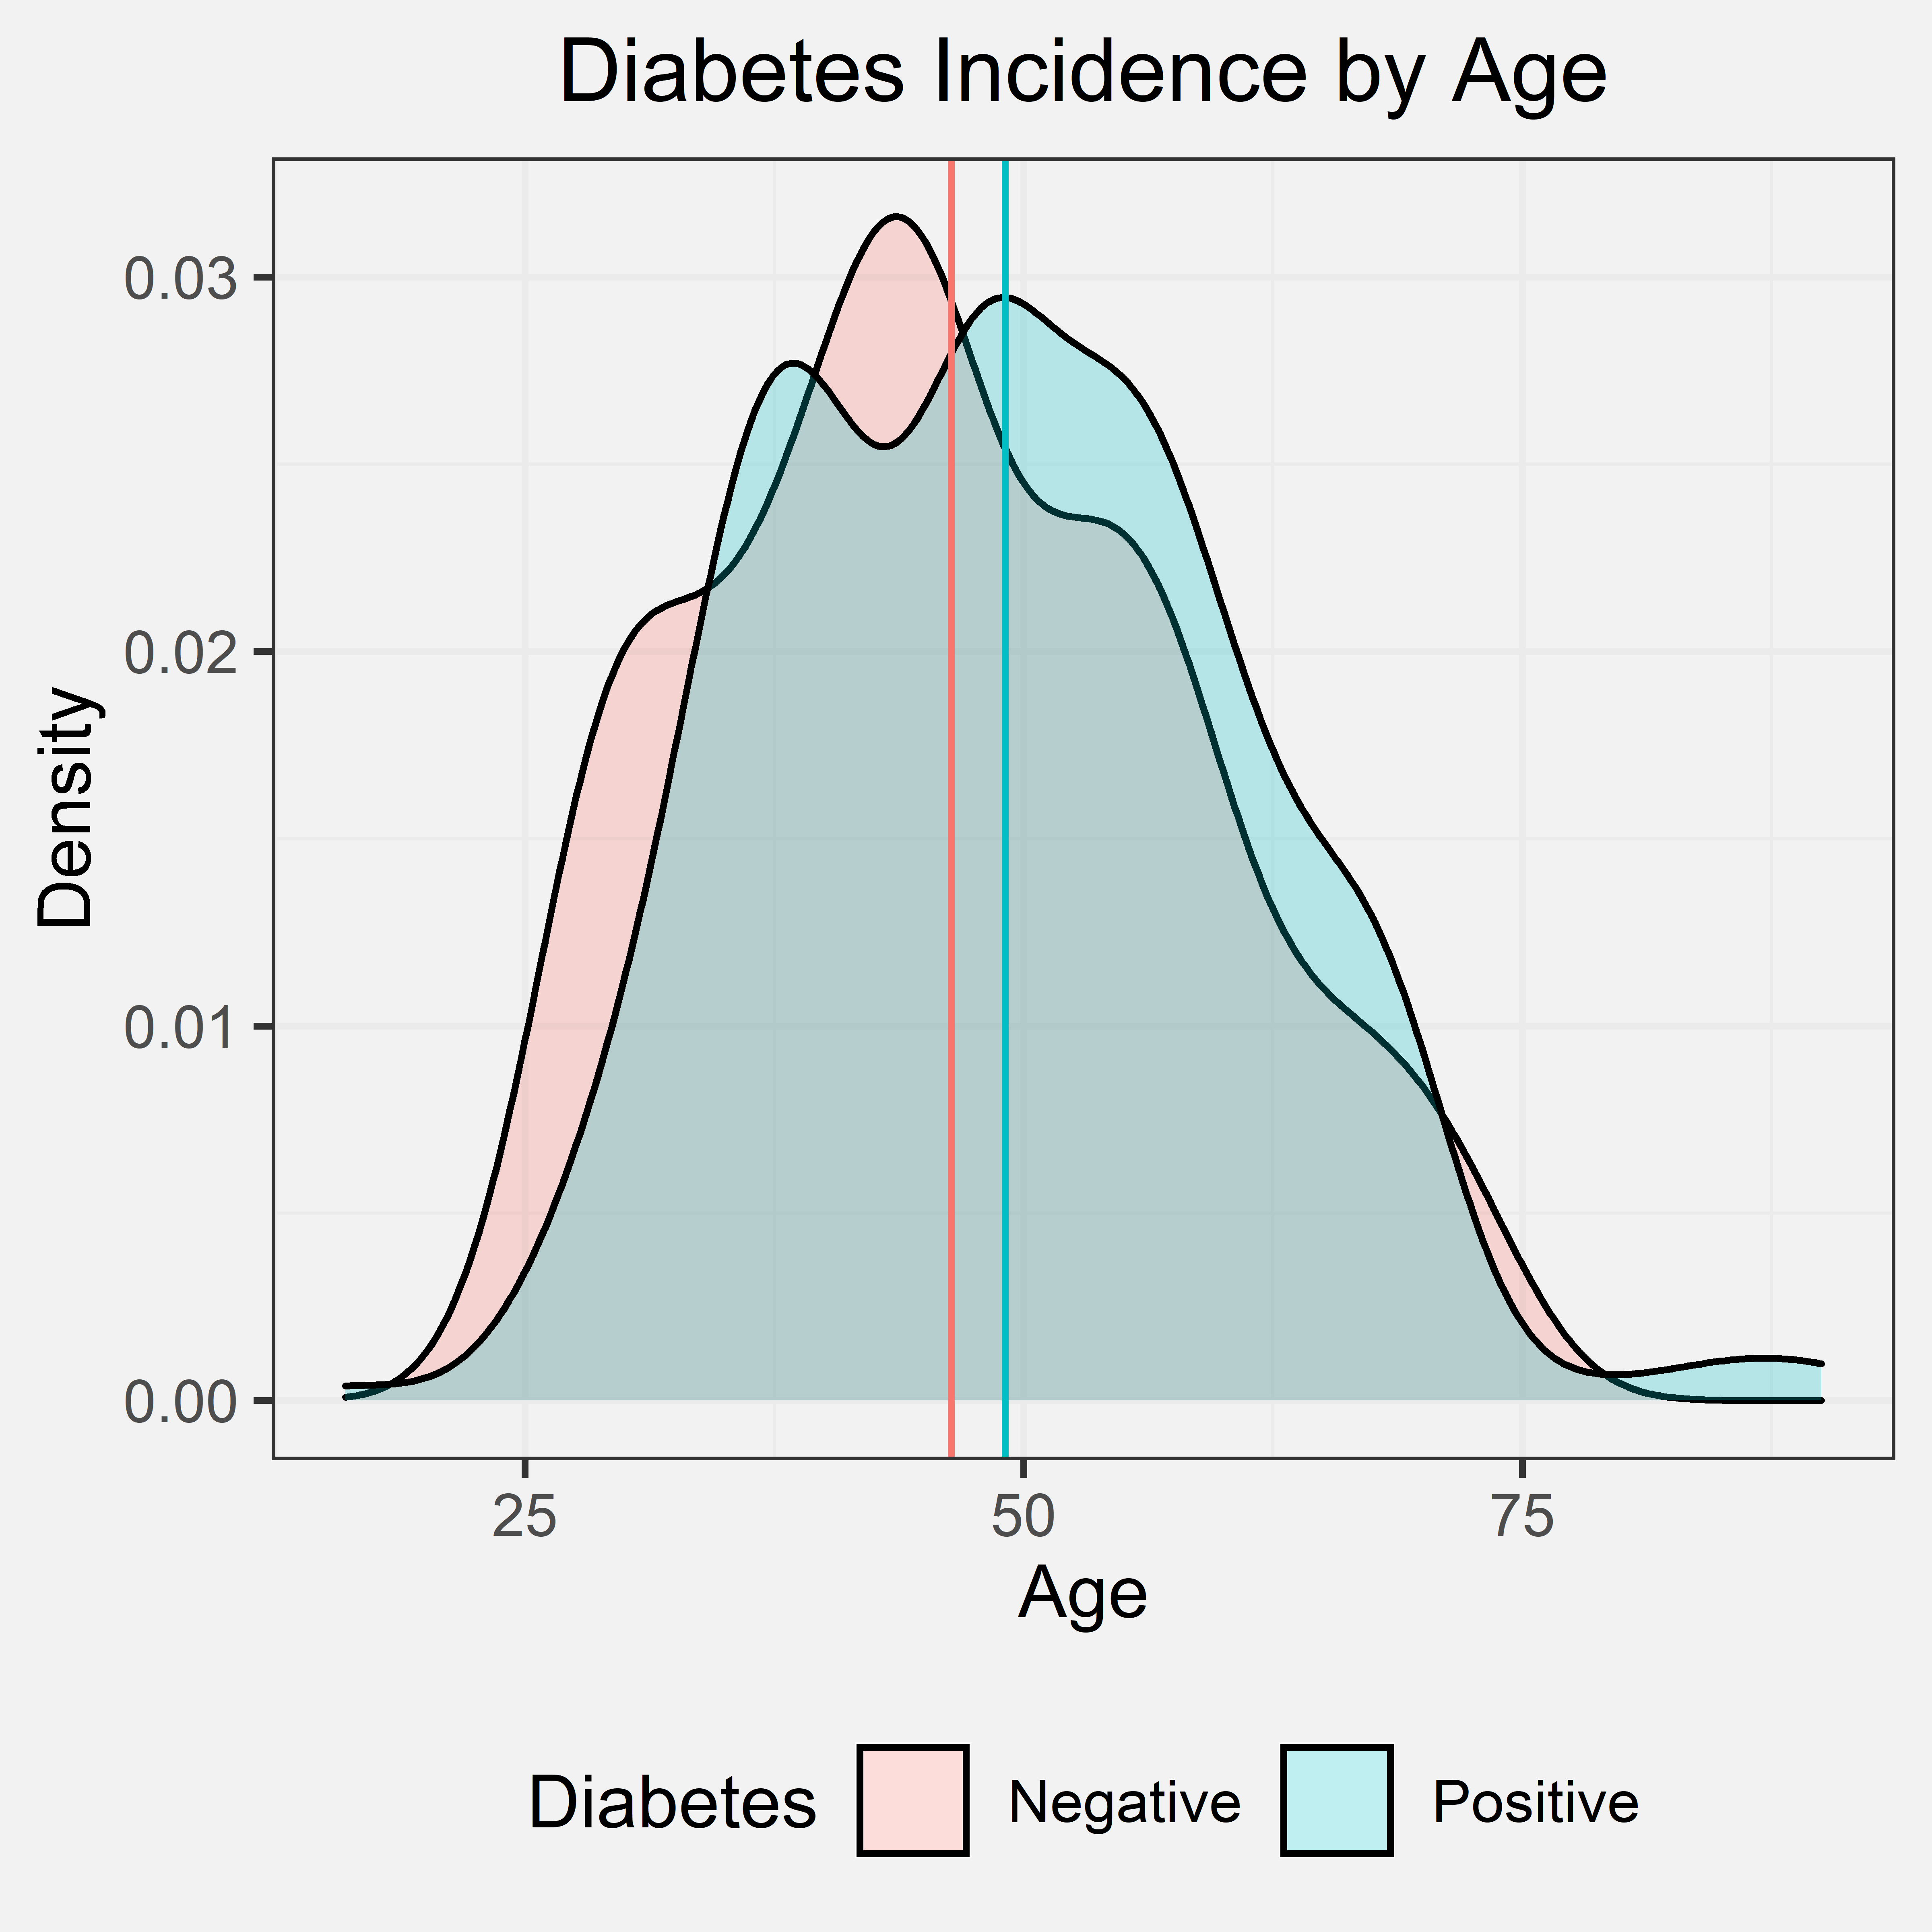
\includegraphics{C:/Users/nilve/Documents/GitHub/diabetes-data-diving/plots/Diabetes_Incidence_by_Age.png}
\caption{Age Density Plot}
\end{figure}

\hypertarget{header-n869}{%
\subsubsection{Conclusion}\label{header-n869}}

From the density graph and the indicated mean ages of patients with and
without diabetes, we can tell that there is only a slightly higher
average age for patients with diabetes and patients without diabetes.
This shows that age is likely not a significant factor for diabetes.
However, the data was collected at a diabetes hospital and did not
account for diabetes type as a potential confounding variable. We cannot
make any significant conclusions, but either way, the density graph does
not support our initial hypothesis.

\hypertarget{header-n871}{%
\subsection{Gender}\label{header-n871}}

\hypertarget{header-n872}{%
\subsubsection{Initial Hypothesis}\label{header-n872}}

Gender was only characterized by two distinct sexes: male and female.
Our initial hypothesis was that gender would have not effect on chances
of diabetes in which the primary basis for this hypothesis was prior
knowledge. Therefore, we expect to see the proportion of diabetes to be
fairly even between the two genders. Out of 520 patients interviewed,
328 were male and 192 were female.

\hypertarget{header-n874}{%
\subsubsection{Bar Chart}\label{header-n874}}

\begin{figure}
\centering
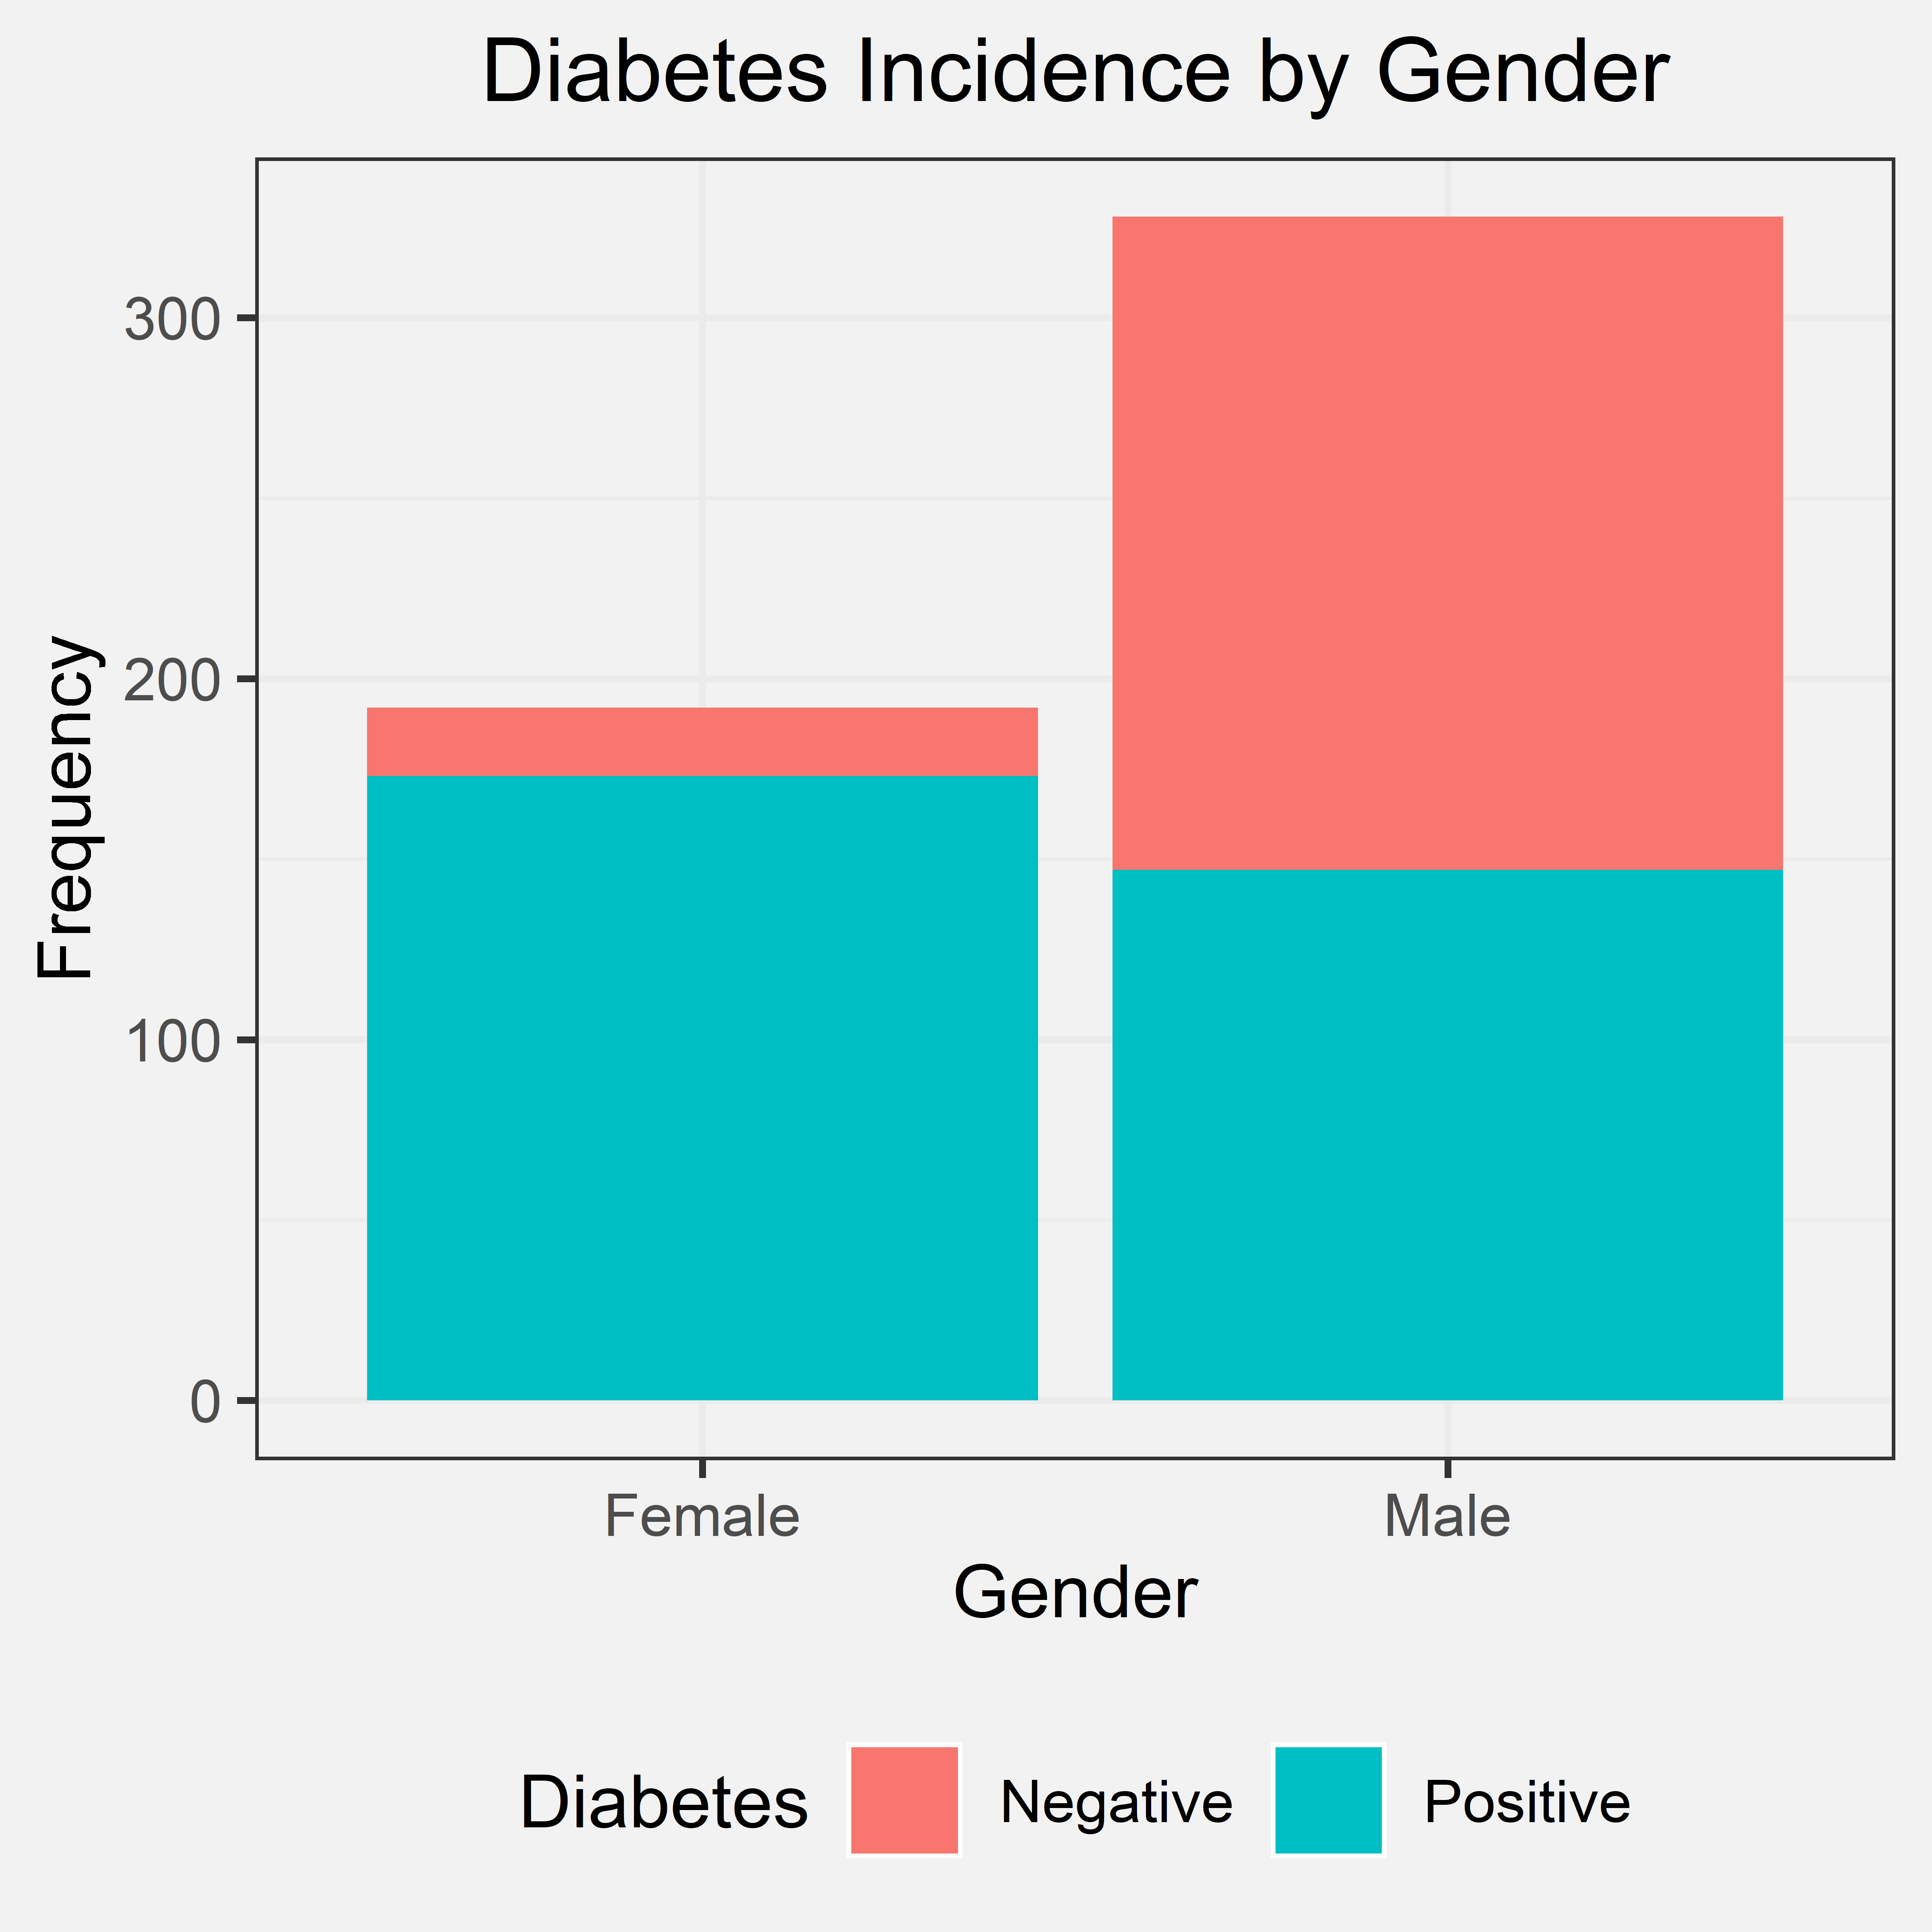
\includegraphics{C:/Users/nilve/Documents/GitHub/diabetes-data-diving/plots/Diabetes_Incidence_by_Gender.png}
\caption{Diabetes Incidence by Gender}
\end{figure}

\hypertarget{header-n876}{%
\subsubsection{Conclusion}\label{header-n876}}

From the bar chart, the frequency of male patients was far greater than
the frequency of female patients. In this dataset, the majority of the
patients with diabetes are female overall, despite how the frequency of
male patients outnumber female patients in the dataset in total. Within
the female patients, an overwhelming majority of the females were
diagnosed with diabetes unlike and in comparison to the male patients in
the dataset. The bar chart does not support our initial hypothesis,
though it seems that female patients have a higher risk for diabetes
with gender as a possible indicator for diabetes as a whole.

\hypertarget{header-n878}{%
\subsection{Polyuria}\label{header-n878}}

\hypertarget{header-n879}{%
\subsubsection{Initial Hypothesis}\label{header-n879}}

Polyuria is the production of abnormally large volumes of dilute urine.
Our initial hypothesis was that if the patient experienced polyuria,
they have a higher chance of being diagnosed with diabetes. We came to
this initial hypothesis through some research and prior knowledge. If an
individual has diabetes, they tend to have higher blood sugar levels,
and their kidney will try to filter out their high blood sugar levels.
This produces a lot of excess urine, leading to polyuria. Out of the 520
patients that were interviewed, 258 had polyuria and 262 did not have
polyuria.

\hypertarget{header-n881}{%
\subsubsection{Bar Chart}\label{header-n881}}

\begin{figure}
\centering
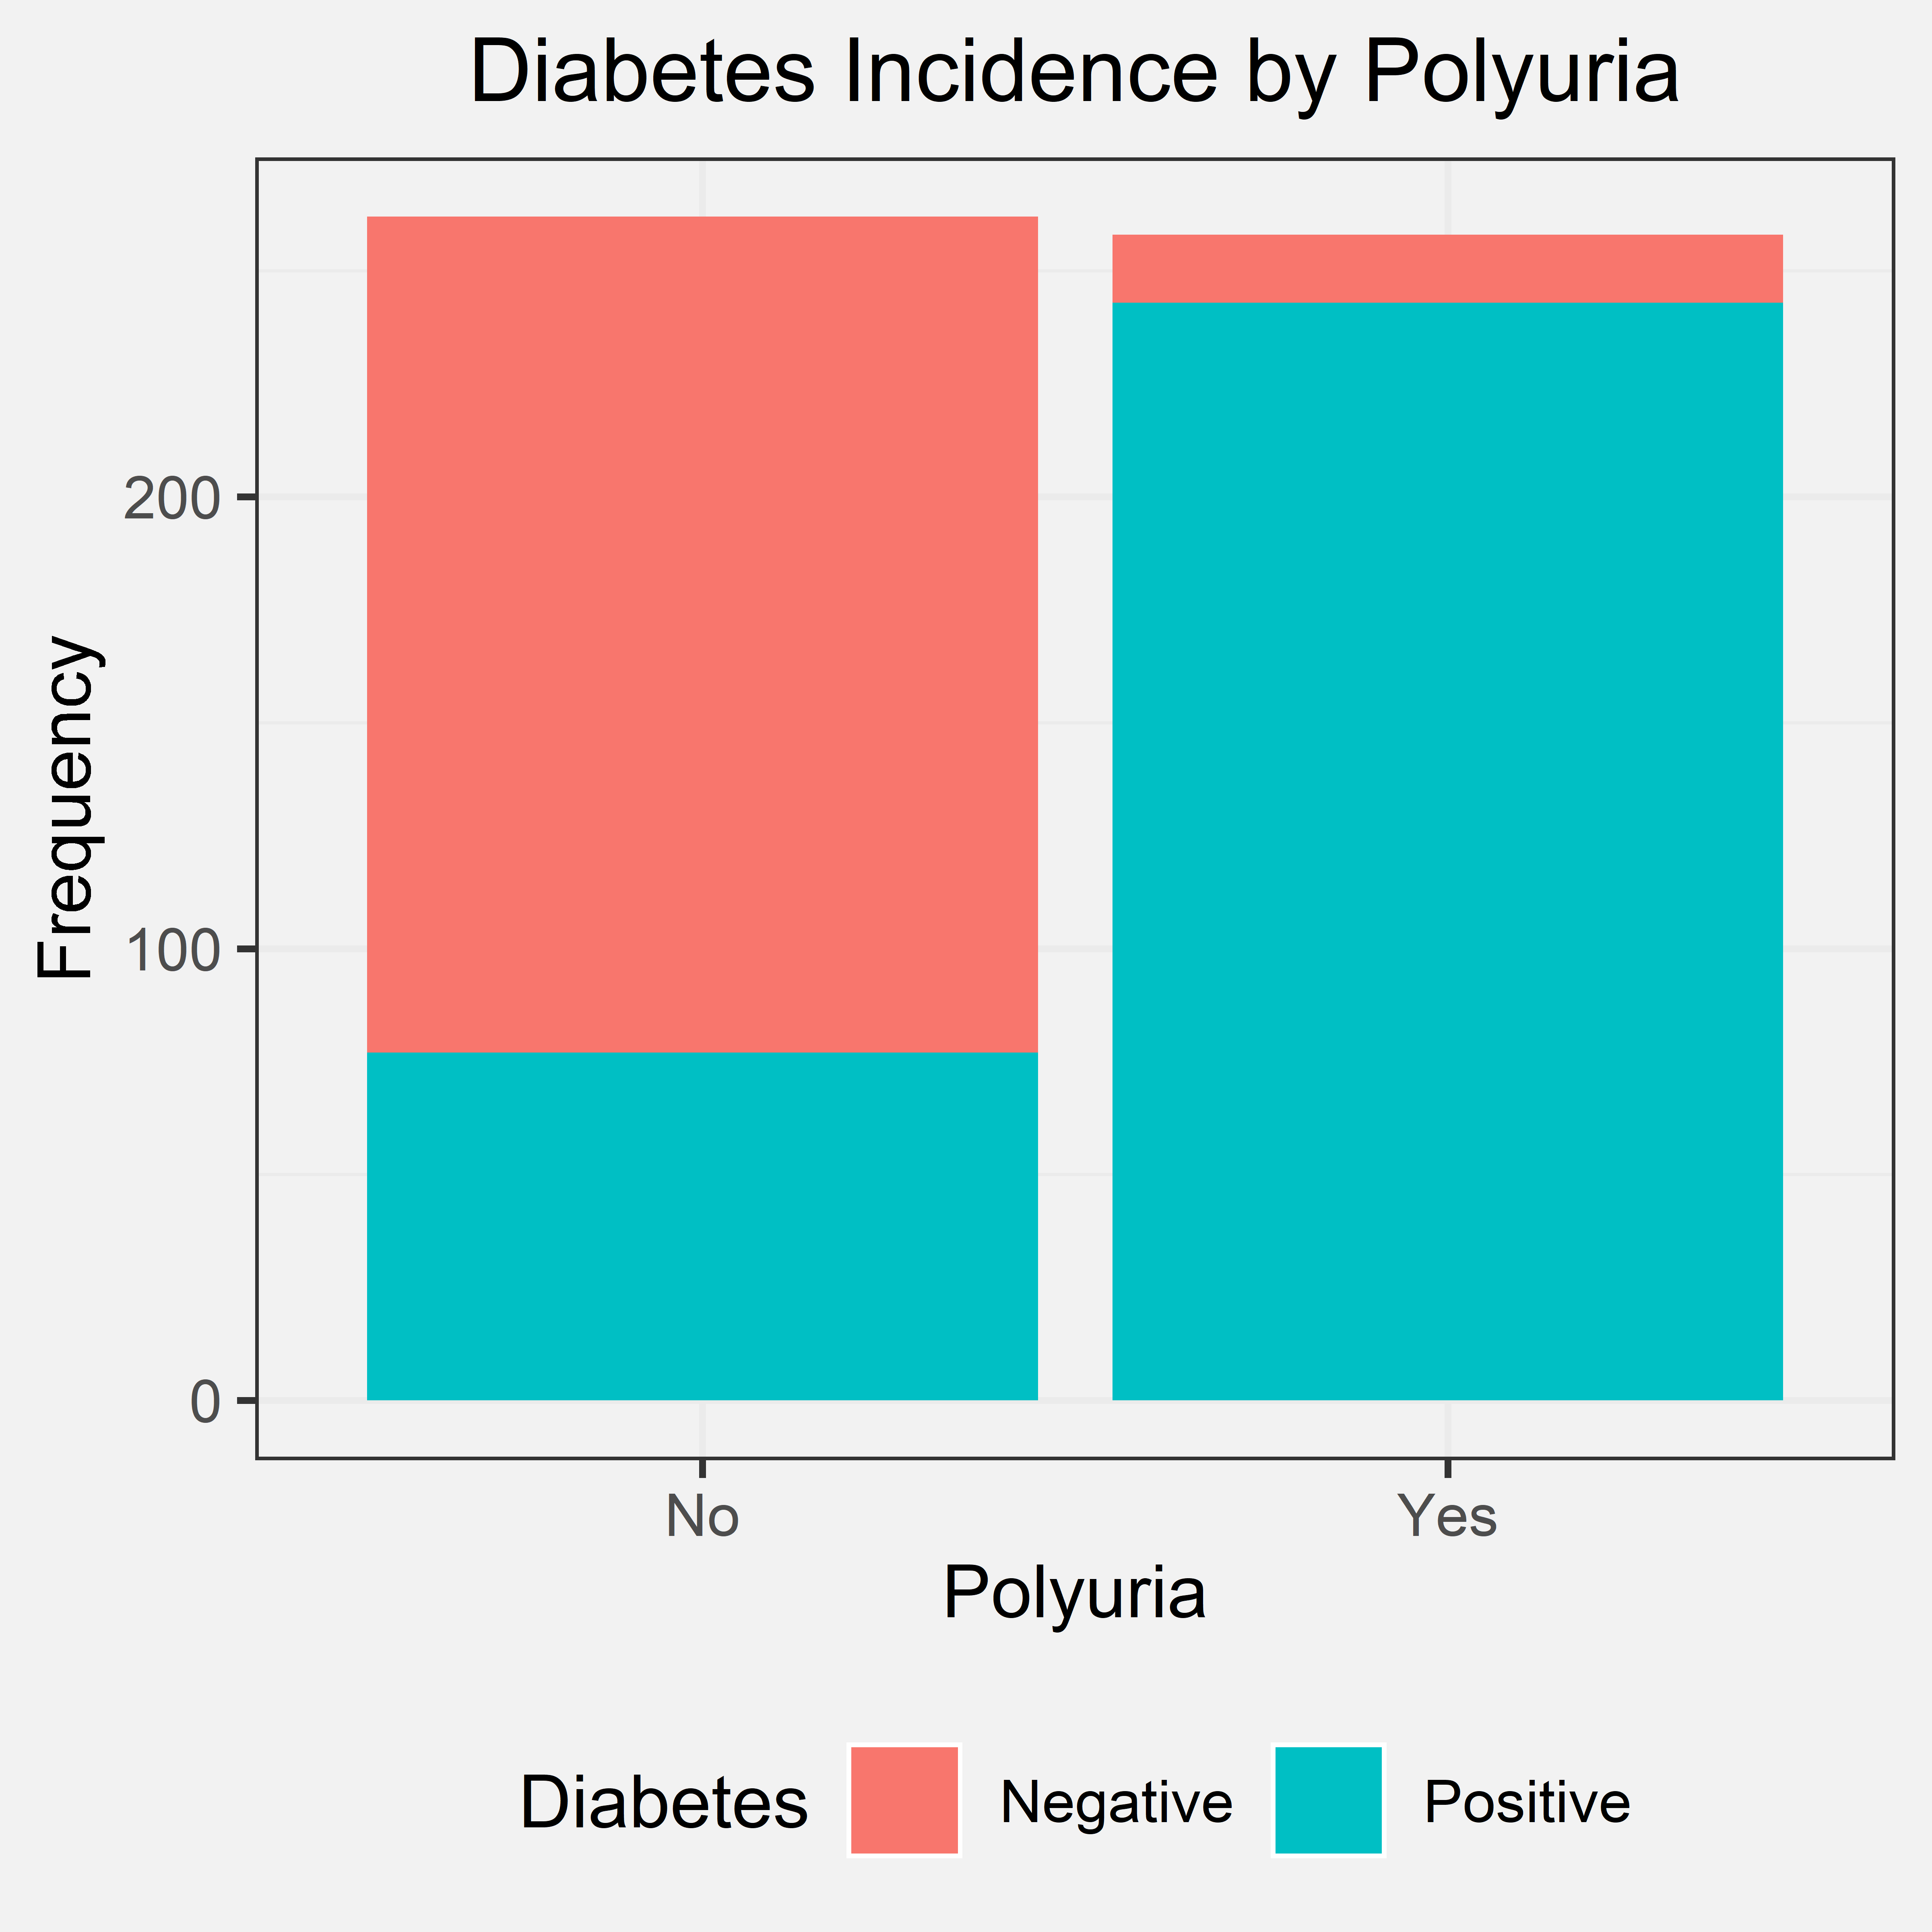
\includegraphics{C:/Users/nilve/Documents/GitHub/diabetes-data-diving/plots/Diabetes_Incidence_by_Polyuria.png}
\caption{Diabetes Incidence by Polyuria}
\end{figure}

\hypertarget{header-n883}{%
\subsubsection{Conclusion}\label{header-n883}}

From the bar chart, we can tell that a great number of individuals who
were diagnosed with diabetes experienced polyuria. A few patients that
were not diagnosed with diabetes also experienced polyuria, but there
was a greater difference in the frequencies in the two situations. Due
to this great difference, we can conclude that nearly all patients with
polyuria have diabetes. Therefore, if a patient experiences polyuria,
they have a higher chance of being diagnosed with diabetes. This shows
us that a possible predictor/indicator for whether an individual has
diabetes should be polyuria. Our bar chart also agreed with our initial
hypothesis.

\hypertarget{header-n885}{%
\subsection{Polydipsia}\label{header-n885}}

\hypertarget{header-n886}{%
\subsubsection{Initial Hypothesis}\label{header-n886}}

Polydipsia is another term for abnormally excessive thirst. Our initial
hypothesis for polydipsia was that if an individual experienced
polydipsia, then they have a much higher chance of being diagnosed with
diabetes. We came to this hypothesis through prior knowledge. Excessive
urine production or polyuria can lead to excessive thirst or polydipsia.
When the body produces these high levels of sugar within the body, the
body will produce increased levels of urine to get rid of excess sugar.
Due to this increased level of urine production, it can lead to
dehydration within the body leading to polydipsia. Out of the 520
patients that were interviewed, 233 said "yes" to experiencing
polydipsia, and 287 said "no".

\hypertarget{header-n888}{%
\subsubsection{Bar Chart}\label{header-n888}}

\begin{figure}
\centering
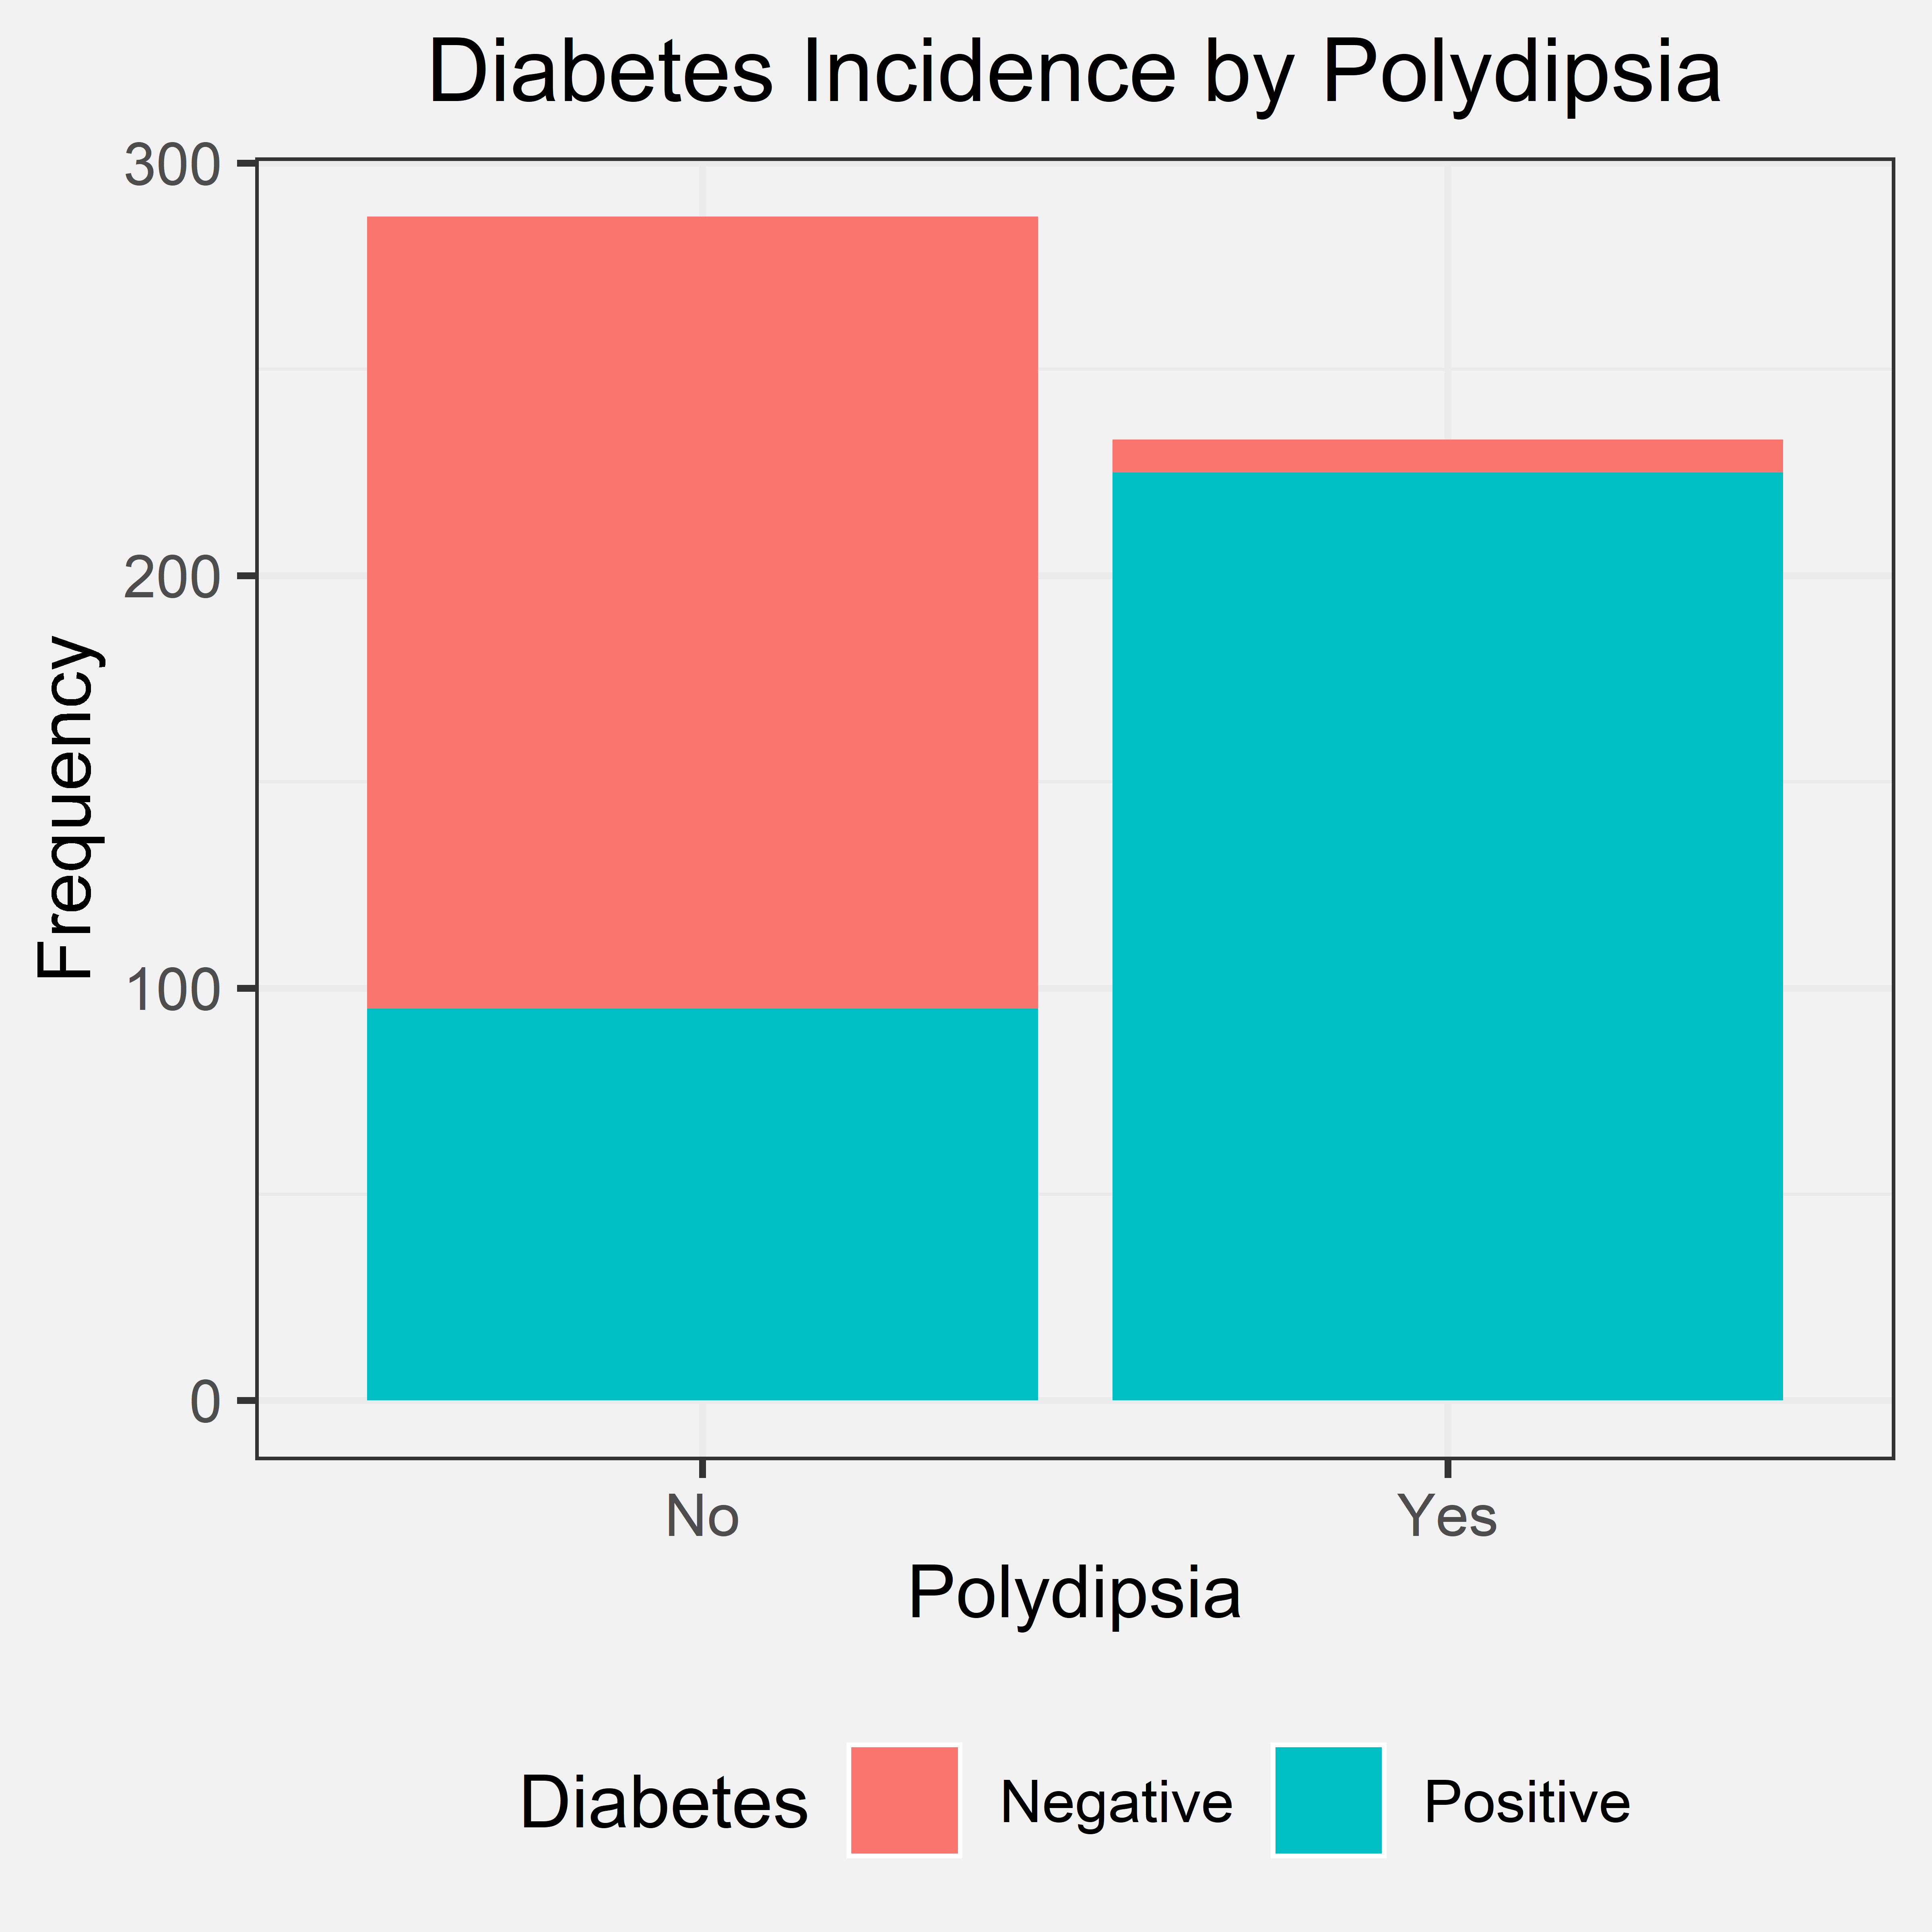
\includegraphics{C:/Users/nilve/Documents/GitHub/diabetes-data-diving/plots/Diabetes_Incidence_by_Polydipsia.png}
\caption{Diabetes Incidence by Polydipsia}
\end{figure}

\hypertarget{header-n890}{%
\subsubsection{Conclusion}\label{header-n890}}

By looking at the bar chart, we can see that nearly all patients that
experienced polydipsia were diagnosed with diabetes. Some individuals
that said "no", were also diagnosed with diabetes. However, almost every
individual that said "yes" to polydipsia was later diagnosed with
diabetes. We concluded that nearly all patients with polydipsia have
diabetes. Therefore, if a patient experiences polydipsia, they have a
higher chance of being diagnosed with diabetes. This conclusion and the
bar chart support our initial hypothesis because a patient having
polydipsia is an important indicator that they might also have a
diagnosis. Therefore, polydipsia can be used as a predictor/indicator
for diabetes due to these patterns.

\hypertarget{header-n892}{%
\subsection{Sudden Weight Loss}\label{header-n892}}

\hypertarget{header-n893}{%
\subsubsection{Initial Hypothesis}\label{header-n893}}

Our initial hypothesis for sudden weight loss was that if an individual
had recently experienced sudden weight loss, then they have a much
higher chance of being diagnosed with diabetes. We came to this
hypothesis due to prior knowledge. Insufficient insulin prevents the
body from getting glucose from the blood into the body's cells to use as
energy. Due to the body not having this instant source of energy, the
body must instead use stored fat within the body as a way to get energy.
The body starts to burn fat and muscle for energy, causing a reduction
in overall body weight. Therefore, we believe that if a patient
experiences sudden weight loss, then they have a high chance of being
diagnosed with diabetes. Out of the 520 patients that were interviewed,
217 experienced sudden weight loss, and 303 did not.

\hypertarget{header-n895}{%
\subsubsection{Bar Chart}\label{header-n895}}

\begin{figure}
\centering
\includegraphics{C:/Users/nilve/Documents/GitHub/diabetes-data-diving/plots/Diabetes_Incidence_by_Sudden_Weight_Loss.png}
\caption{Diabetes Incidence by Sudden Weight Loss}
\end{figure}

\hypertarget{header-n897}{%
\subsubsection{Conclusion}\label{header-n897}}

From the bar chart, we can see that a loss of individuals that said yes
to experiencing sudden weight loss also was diagnosed with diabetes.
There were a few who experienced sudden weight loss and were still not
diagnosed with diabetes. Several individuals did not experience sudden
weight loss and were still diagnosed with diabetes. Even though, sudden
weight loss has a smaller amount of difference between the two values
compared to polydipsia and polyuria; however, there is still a
significant difference. Therefore, we concluded that if a patient has
had sudden weight loss, it is very likely that they have diabetes, but
the converse is not true. We did not include the second part within the
initial hypothesis because we did not think about the pattern for the
converse. However, the first part of our conclusion agrees with our
initial hypothesis. Therefore, sudden weight loss can be used as a
predictor/indicator of whether the patient will have diabetes or not.

\hypertarget{header-n899}{%
\subsection{Partial Paresis}\label{header-n899}}

\hypertarget{header-n900}{%
\subsubsection{Initial Hypothesis}\label{header-n900}}

Paresis is a condition typifies by a weakness of the voluntary movement.
We came up with the initial hypothesis that if the individual has
partial paresis, then they have a much higher chance of being diagnosed
with diabetes. We came up with this hypothesis by using prior knowledge.
Diabetes can sometimes lead to nerve damage which can lead to partial
paresis in some cases, so we believed that there would be some sort of
correlation between the two. 224 patients said "yes" to experiencing
partial paresis, and 296 said "no" out of the 520 patients.

\hypertarget{header-n902}{%
\subsubsection{Bar Chart}\label{header-n902}}

\begin{figure}
\centering
\includegraphics{C:/Users/nilve/Documents/GitHub/diabetes-data-diving/plots/Diabetes_Incidence_by_Partial_Paresis.png}
\caption{Diabetes Incidence by Partial Paresis}
\end{figure}

\hypertarget{header-n904}{%
\subsubsection{Conclusion}\label{header-n904}}

According to the bar chart most of the patients that said "yes" to
partial paresis were diagnosed with diabetes. There were still several
patients that said "no" to partial paresis and still were diagnosed with
diabetes. The conclusion we came to was that if a patient has partial
paresis, it is very likely that they have diabetes, but the converse is
not true. This conclusion supports our initial hypothesis. Our initial
hypothesis did not mention the converse; however, the first part of our
conclusion still supports our initial hypothesis.

\hypertarget{header-n906}{%
\section{Model}\label{header-n906}}

For the modelling portion of our project, we compared two different
types of models. For our simple model, we tried out a linear regression.
For our complex model, we implemented a random forest classifier.

\hypertarget{header-n908}{%
\subsection{Linear Regression Model}\label{header-n908}}

\hypertarget{header-n909}{%
\subsubsection{Loading in Data}\label{header-n909}}

This notebook will be focused on building a predictive model from the
dataset. The response variable is class, and all other variables are
predictors. All predictors are categorical except for Age which is a
ordinal variable. In the encoding below, ``Yes'' is 1 and ``No'' is 0.
Additionally, ``Male'' is 0 and ``Female'' is 1 for the Gender column.

\begin{Shaded}
\begin{Highlighting}[]
\KeywordTok{require}\NormalTok{(tidyverse)}
\KeywordTok{set.seed}\NormalTok{(}\DecValTok{100}\NormalTok{)}

\NormalTok{data <-}\StringTok{ }\KeywordTok{read_csv}\NormalTok{(}\StringTok{"../data/clean_numeric_data.csv"}\NormalTok{)}
\KeywordTok{head}\NormalTok{(data)}
\end{Highlighting}
\end{Shaded}

\begin{verbatim}
## # A tibble: 6 x 17
##     Age Gender Polyuria Polydipsia sudden.weight.l~ weakness Polyphagia
##   <dbl>  <dbl>    <dbl>      <dbl>            <dbl>    <dbl>      <dbl>
## 1    40      0        0          1                0        1          0
## 2    58      0        0          0                0        1          0
## 3    41      0        1          0                0        1          1
## 4    45      0        0          0                1        1          1
## 5    60      0        1          1                1        1          1
## 6    55      0        1          1                0        1          1
## # ... with 10 more variables: Genital.thrush <dbl>, visual.blurring <dbl>,
## #   Itching <dbl>, Irritability <dbl>, delayed.healing <dbl>,
## #   partial.paresis <dbl>, muscle.stiffness <dbl>, Alopecia <dbl>,
## #   Obesity <dbl>, class <dbl>
\end{verbatim}

\hypertarget{header-n913}{%
\subsubsection{Building the linear model}\label{header-n913}}

Using the results of the chi-square feature selection process from
earlier, we will limit the linear regression model to the six variables
we investigated above.

\begin{Shaded}
\begin{Highlighting}[]
\CommentTok{# building the linear model}
\NormalTok{model <-}\StringTok{ }\KeywordTok{lm}\NormalTok{(class }\OperatorTok{~}\StringTok{ }\NormalTok{Age }\OperatorTok{+}\StringTok{ }\NormalTok{Gender }\OperatorTok{+}\StringTok{ }\NormalTok{Polyuria }\OperatorTok{+}\StringTok{ }\NormalTok{Polydipsia }\OperatorTok{+}\StringTok{ }\NormalTok{sudden.weight.loss }\OperatorTok{+}\StringTok{ }\NormalTok{partial.paresis, }\DataTypeTok{data=}\NormalTok{data)}

\KeywordTok{summary}\NormalTok{(model)}
\end{Highlighting}
\end{Shaded}

\begin{verbatim}
## 
## Call:
## lm(formula = class ~ Age + Gender + Polyuria + Polydipsia + sudden.weight.loss + 
##     partial.paresis, data = data)
## 
## Residuals:
##     Min      1Q  Median      3Q     Max 
## -0.6059 -0.1747 -0.1662  0.1614  0.8311 
## 
## Coefficients:
##                      Estimate Std. Error t value Pr(>|t|)    
## (Intercept)         0.1885380  0.0580208   3.249  0.00123 ** 
## Age                -0.0003632  0.0011812  -0.307  0.75864    
## Gender              0.2190474  0.0314266   6.970 9.77e-12 ***
## Polyuria            0.3623175  0.0367050   9.871  < 2e-16 ***
## Polydipsia          0.3052143  0.0361974   8.432 3.47e-16 ***
## sudden.weight.loss  0.0710132  0.0319390   2.223  0.02662 *  
## partial.paresis     0.0400450  0.0330831   1.210  0.22667    
## ---
## Signif. codes:  0 '***' 0.001 '**' 0.01 '*' 0.05 '.' 0.1 ' ' 1
## 
## Residual standard error: 0.3113 on 513 degrees of freedom
## Multiple R-squared:  0.596,  Adjusted R-squared:  0.5913 
## F-statistic: 126.1 on 6 and 513 DF,  p-value: < 2.2e-16
\end{verbatim}

From the summary of the model, we see that all the variables have
p-values\textless{}0.05, indicating statistically significant
relationships, except for Age and Partial Paresis. Additionally, all
variables except for Age have a positive slope which makes sense given
that our bar charts show that answering ``Yes'' for these risk factors
or being female makes it much more likely for a patient to have
diabetes.

We can also calculate the following performance metrics for our model.

\hypertarget{header-n919}{%
\paragraph{Mean Squared Prediction Error (MSPE)}\label{header-n919}}

\begin{Shaded}
\begin{Highlighting}[]
\KeywordTok{mean}\NormalTok{(model}\OperatorTok{$}\NormalTok{residual}\OperatorTok{^}\DecValTok{2}\NormalTok{)}
\end{Highlighting}
\end{Shaded}

\begin{verbatim}
## [1] 0.09561477
\end{verbatim}

\hypertarget{header-n922}{%
\paragraph{\texorpdfstring{Coefficient of Determination
(\(R^2\))}{Coefficient of Determination (R\^{}2)}}\label{header-n922}}

\begin{Shaded}
\begin{Highlighting}[]
\KeywordTok{summary}\NormalTok{(model)}\OperatorTok{$}\NormalTok{r.squared }
\end{Highlighting}
\end{Shaded}

\begin{verbatim}
## [1] 0.5960276
\end{verbatim}

\hypertarget{header-n925}{%
\subsubsection{Checking Assumptions}\label{header-n925}}

For a linear model, we first check to see if the relationships in the
linear model are independent. These risk factors in the dataset are not
necessarily independent. In particular, as evidenced from the
correlation heatmap plot from earlier, polydipsia and polyuria are
highly correlated with each other. They also have a biological link. The
independence assumption of the linear model is not met.

Residual Plot:

\begin{Shaded}
\begin{Highlighting}[]
\NormalTok{mod_results <-}\StringTok{ }\KeywordTok{data.frame}\NormalTok{(}\DataTypeTok{observed =}\NormalTok{ data}\OperatorTok{$}\NormalTok{class, 
}
                          \DataTypeTok{predicted =}\NormalTok{ model}\OperatorTok{$}\NormalTok{fitted.values, 
}
                          \DataTypeTok{residual =}\NormalTok{ model}\OperatorTok{$}\NormalTok{residuals)
}
\KeywordTok{head}\NormalTok{(mod_results)}
\end{Highlighting}
\end{Shaded}

\begin{verbatim}
##   observed predicted   residual
## 1        1 0.4792263 0.52077365
## 2        1 0.2075204 0.79247964
## 3        1 0.5359663 0.46403365
## 4        1 0.2432095 0.75679047
## 5        1 0.9453391 0.05466093
## 6        1 0.8360966 0.16390344
\end{verbatim}

\begin{Shaded}
\begin{Highlighting}[]
\KeywordTok{ggplot}\NormalTok{(mod_results, }\KeywordTok{aes}\NormalTok{(}\DataTypeTok{y =}\NormalTok{ residual, }\DataTypeTok{x =}\NormalTok{ predicted)) }\OperatorTok{+}\StringTok{ }
\StringTok{    }\KeywordTok{geom_point}\NormalTok{() }\OperatorTok{+}\StringTok{ }
\StringTok{    }\KeywordTok{geom_hline}\NormalTok{(}\DataTypeTok{yintercept =} \DecValTok{0}\NormalTok{) }\OperatorTok{+}
\StringTok{      }\KeywordTok{theme_bw}\NormalTok{() }\OperatorTok{+}
\StringTok{  }\KeywordTok{labs}\NormalTok{(}\DataTypeTok{title=}\StringTok{"Residual Plot"}\NormalTok{, }\DataTypeTok{x=}\StringTok{"Predicted"}\NormalTok{, }\DataTypeTok{y=}\StringTok{"Residual"}\NormalTok{) }\OperatorTok{+}
\StringTok{  }\KeywordTok{theme}\NormalTok{(}\DataTypeTok{plot.title =} \KeywordTok{element_text}\NormalTok{(}\DataTypeTok{hjust =} \FloatTok{0.5}\NormalTok{)) }\OperatorTok{+}
\StringTok{  }\KeywordTok{theme}\NormalTok{(}\DataTypeTok{plot.background =} \KeywordTok{element_rect}\NormalTok{(}\DataTypeTok{fill =} \StringTok{'#f2f2f2'}\NormalTok{, }\DataTypeTok{colour =} \StringTok{'#f2f2f2'}\NormalTok{)) }\OperatorTok{+}
\StringTok{  }\KeywordTok{theme}\NormalTok{(}\DataTypeTok{panel.background =} \KeywordTok{element_rect}\NormalTok{(}\DataTypeTok{fill =} \StringTok{'#f2f2f2'}\NormalTok{, }\DataTypeTok{colour =} \StringTok{'#f2f2f2'}\NormalTok{))}
\end{Highlighting}
\end{Shaded}

\begin{figure}
\centering
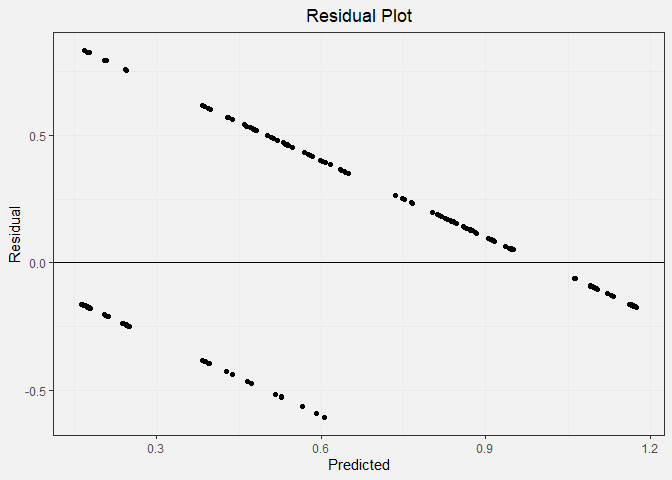
\includegraphics{C:/Users/nilve/Documents/GitHub/diabetes-data-diving/notebooks/linear_model_files/figure-gfm/residual-1.png}
\caption{}
\end{figure}

In the residual plot, we expect to see symmetrically distributed points
forming a cloud. We also hope to see low residual values and no clear
patterns. This is not the case for our data because the output must be a
0 or a 1. This causes the linear regression model to form two
distinctive lines on the plot.

Q-Q Plot:

\begin{Shaded}
\begin{Highlighting}[]
\KeywordTok{ggplot}\NormalTok{(mod_results, }\KeywordTok{aes}\NormalTok{(}\DataTypeTok{sample =}\NormalTok{ residual)) }\OperatorTok{+}\StringTok{ }
\StringTok{    }\KeywordTok{geom_qq}\NormalTok{()}\OperatorTok{+}
\StringTok{  }\KeywordTok{geom_qq_line}\NormalTok{() }\OperatorTok{+}
\StringTok{  }\KeywordTok{theme_bw}\NormalTok{() }\OperatorTok{+}
\StringTok{  }\KeywordTok{labs}\NormalTok{(}\DataTypeTok{title=}\StringTok{"Q-Q Plot"}\NormalTok{, }\DataTypeTok{x=}\StringTok{"Theoretical Quantile"}\NormalTok{, }\DataTypeTok{y=}\StringTok{"Sample Quantile"}\NormalTok{) }\OperatorTok{+}
\StringTok{  }\KeywordTok{theme}\NormalTok{(}\DataTypeTok{plot.title =} \KeywordTok{element_text}\NormalTok{(}\DataTypeTok{hjust =} \FloatTok{0.5}\NormalTok{)) }\OperatorTok{+}
\StringTok{  }\KeywordTok{theme}\NormalTok{(}\DataTypeTok{plot.background =} \KeywordTok{element_rect}\NormalTok{(}\DataTypeTok{fill =} \StringTok{'#f2f2f2'}\NormalTok{, }\DataTypeTok{colour =} \StringTok{'#f2f2f2'}\NormalTok{)) }\OperatorTok{+}
\StringTok{  }\KeywordTok{theme}\NormalTok{(}\DataTypeTok{panel.background =} \KeywordTok{element_rect}\NormalTok{(}\DataTypeTok{fill =} \StringTok{'#f2f2f2'}\NormalTok{, }\DataTypeTok{colour =} \StringTok{'#f2f2f2'}\NormalTok{))}
\end{Highlighting}
\end{Shaded}

\begin{figure}
\centering
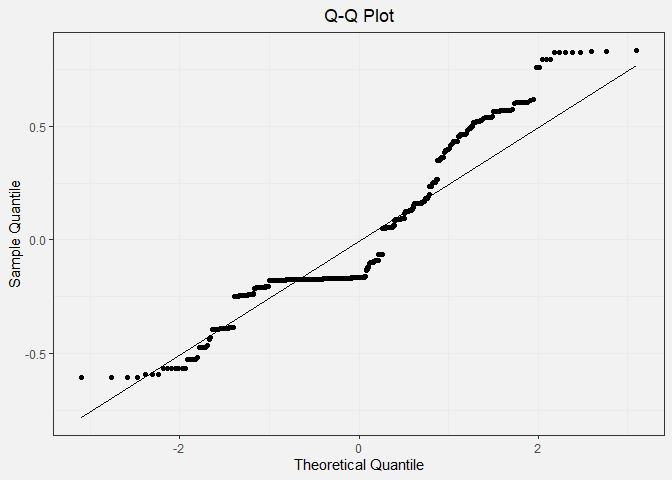
\includegraphics{C:/Users/nilve/Documents/GitHub/diabetes-data-diving/notebooks/linear_model_files/figure-gfm/qq-1.png}
\caption{}
\end{figure}

In the Q-Q plot, we expect to see the points in the scatter plot to
closely follow the diagonal line. This pattern is clearly not observed.

The mean and standard deviation for our residuals can be calculated as
such:

\begin{Shaded}
\begin{Highlighting}[]
\NormalTok{mean_res <-}\StringTok{ }\KeywordTok{mean}\NormalTok{(mod_results}\OperatorTok{$}\NormalTok{residual)}
\NormalTok{sd_res <-}\StringTok{ }\KeywordTok{sd}\NormalTok{(mod_results}\OperatorTok{$}\NormalTok{residual)}
\KeywordTok{print}\NormalTok{(}\KeywordTok{c}\NormalTok{(mean_res, sd_res))}
\end{Highlighting}
\end{Shaded}

\begin{verbatim}
## [1] -2.469760e-17  3.095141e-01
\end{verbatim}

\hypertarget{header-n942}{%
\subsubsection{Conclusion}\label{header-n942}}

Overall, our assumptions are not met, and a linear regression model is
not a good way to model our data.

\hypertarget{header-n944}{%
\subsection{Random Forest Model}\label{header-n944}}

\hypertarget{header-n945}{%
\subsubsection{Loading Random Forest Libraries}\label{header-n945}}

\begin{Shaded}
\begin{Highlighting}[]
\KeywordTok{require}\NormalTok{(randomForest)}
\KeywordTok{require}\NormalTok{(caTools)}
\KeywordTok{require}\NormalTok{(tidyverse)}

\KeywordTok{set.seed}\NormalTok{(}\DecValTok{2020}\NormalTok{)}
\end{Highlighting}
\end{Shaded}

\hypertarget{header-n947}{%
\subsubsection{Loading in Data}\label{header-n947}}

We can read in the data using the \texttt{read\_csv()} function. The
parameters included in this function are to transform the categorical
data into factor data types for easy analysis later on.

\begin{Shaded}
\begin{Highlighting}[]
\NormalTok{diabetes_data_upload <-}\StringTok{ }\KeywordTok{read_csv}\NormalTok{(}
  \StringTok{"../data/diabetes_data_upload.csv"}\NormalTok{,}
  \DataTypeTok{col_types =} \KeywordTok{cols}\NormalTok{(}
    \DataTypeTok{Gender =} \KeywordTok{col_factor}\NormalTok{(}\DataTypeTok{levels =} \KeywordTok{c}\NormalTok{(}\StringTok{"Male"}\NormalTok{, }\StringTok{"Female"}\NormalTok{)),}
    \DataTypeTok{Polyuria =} \KeywordTok{col_factor}\NormalTok{(}\DataTypeTok{levels =} \KeywordTok{c}\NormalTok{(}\StringTok{"Yes"}\NormalTok{, }\StringTok{"No"}\NormalTok{)),}
    \DataTypeTok{Polydipsia =} \KeywordTok{col_factor}\NormalTok{(}\DataTypeTok{levels =} \KeywordTok{c}\NormalTok{(}\StringTok{"Yes"}\NormalTok{, }\StringTok{"No"}\NormalTok{)),}
    \StringTok{`}\DataTypeTok{sudden weight loss}\StringTok{`}\NormalTok{ =}\StringTok{ }\KeywordTok{col_factor}\NormalTok{(}\DataTypeTok{levels =} \KeywordTok{c}\NormalTok{(}\StringTok{"Yes"}\NormalTok{, }\StringTok{"No"}\NormalTok{)),}
    \DataTypeTok{weakness =} \KeywordTok{col_factor}\NormalTok{(}\DataTypeTok{levels =} \KeywordTok{c}\NormalTok{(}\StringTok{"Yes"}\NormalTok{, }\StringTok{"No"}\NormalTok{)),}
    \DataTypeTok{Polyphagia =} \KeywordTok{col_factor}\NormalTok{(}\DataTypeTok{levels =} \KeywordTok{c}\NormalTok{(}\StringTok{"Yes"}\NormalTok{, }\StringTok{"No"}\NormalTok{)),}
    \StringTok{`}\DataTypeTok{Genital thrush}\StringTok{`}\NormalTok{ =}\StringTok{ }\KeywordTok{col_factor}\NormalTok{(}\DataTypeTok{levels =} \KeywordTok{c}\NormalTok{(}\StringTok{"Yes"}\NormalTok{, }\StringTok{"No"}\NormalTok{)),}
    \StringTok{`}\DataTypeTok{visual blurring}\StringTok{`}\NormalTok{ =}\StringTok{ }\KeywordTok{col_factor}\NormalTok{(}\DataTypeTok{levels =} \KeywordTok{c}\NormalTok{(}\StringTok{"Yes"}\NormalTok{, }\StringTok{"No"}\NormalTok{)),}
    \DataTypeTok{Itching =} \KeywordTok{col_factor}\NormalTok{(}\DataTypeTok{levels =} \KeywordTok{c}\NormalTok{(}\StringTok{"Yes"}\NormalTok{, }\StringTok{"No"}\NormalTok{)),}
    \DataTypeTok{Irritability =} \KeywordTok{col_factor}\NormalTok{(}\DataTypeTok{levels =} \KeywordTok{c}\NormalTok{(}\StringTok{"Yes"}\NormalTok{, }\StringTok{"No"}\NormalTok{)),}
    \StringTok{`}\DataTypeTok{delayed healing}\StringTok{`}\NormalTok{ =}\StringTok{ }\KeywordTok{col_factor}\NormalTok{(}\DataTypeTok{levels =} \KeywordTok{c}\NormalTok{(}\StringTok{"Yes"}\NormalTok{, }\StringTok{"No"}\NormalTok{)),}
    \StringTok{`}\DataTypeTok{partial paresis}\StringTok{`}\NormalTok{ =}\StringTok{ }\KeywordTok{col_factor}\NormalTok{(}\DataTypeTok{levels =} \KeywordTok{c}\NormalTok{(}\StringTok{"Yes"}\NormalTok{, }\StringTok{"No"}\NormalTok{)),}
    \StringTok{`}\DataTypeTok{muscle stiffness}\StringTok{`}\NormalTok{ =}\StringTok{ }\KeywordTok{col_factor}\NormalTok{(}\DataTypeTok{levels =} \KeywordTok{c}\NormalTok{(}\StringTok{"Yes"}\NormalTok{, }\StringTok{"No"}\NormalTok{)),}
    \DataTypeTok{Alopecia =} \KeywordTok{col_factor}\NormalTok{(}\DataTypeTok{levels =} \KeywordTok{c}\NormalTok{(}\StringTok{"Yes"}\NormalTok{, }\StringTok{"No"}\NormalTok{)),}
    \DataTypeTok{Obesity =} \KeywordTok{col_factor}\NormalTok{(}\DataTypeTok{levels =} \KeywordTok{c}\NormalTok{(}\StringTok{"Yes"}\NormalTok{, }\StringTok{"No"}\NormalTok{)),}
    \DataTypeTok{class =} \KeywordTok{col_factor}\NormalTok{(}\DataTypeTok{levels =} \KeywordTok{c}\NormalTok{(}\StringTok{"Positive"}\NormalTok{, }\StringTok{"Negative"}\NormalTok{))}
\NormalTok{  )}
\NormalTok{)}

\NormalTok{diabetes_data_upload <-}\StringTok{ }\KeywordTok{data.frame}\NormalTok{(diabetes_data_upload)}

\KeywordTok{summary}\NormalTok{(diabetes_data_upload)}
\end{Highlighting}
\end{Shaded}

\begin{verbatim}
##       Age           Gender    Polyuria  Polydipsia sudden.weight.loss weakness 
##  Min.   :16.00   Male  :328   Yes:258   Yes:233    Yes:217            Yes:305  
##  1st Qu.:39.00   Female:192   No :262   No :287    No :303            No :215  
##  Median :47.50                                                                 
##  Mean   :48.03                                                                 
##  3rd Qu.:57.00                                                                 
##  Max.   :90.00                                                                 
##  Polyphagia Genital.thrush visual.blurring Itching   Irritability
##  Yes:237    Yes:116        Yes:233         Yes:253   Yes:126     
##  No :283    No :404        No :287         No :267   No :394     
##                                                                  
##                                                                  
##                                                                  
##                                                                  
##  delayed.healing partial.paresis muscle.stiffness Alopecia  Obesity  
##  Yes:239         Yes:224         Yes:195          Yes:179   Yes: 88  
##  No :281         No :296         No :325          No :341   No :432  
##                                                                      
##                                                                      
##                                                                      
##                                                                      
##       class    
##  Positive:320  
##  Negative:200  
##                
##                
##                
## 
\end{verbatim}

In the summary of our data, we see that there are more patients with
diabetes than without, which calls into question the validity of our
model. While dataset is unbalanced, 320 vs 200 is not a very large
difference, so our model should still be reasonably accurate.

\hypertarget{header-n952}{%
\subsubsection{Splitting Data into a Training and Testing
Set}\label{header-n952}}

In preparation modeling our data, we can first separate it into a
testing and a training set with a split ratio of 0.8. This means that
80\% of our overall dataset will be used for training and 20\% will be
used for testing the model at the end.

\begin{Shaded}
\begin{Highlighting}[]
\NormalTok{sample =}\StringTok{ }\KeywordTok{sample.split}\NormalTok{(diabetes_data_upload}\OperatorTok{$}\NormalTok{class, }\DataTypeTok{SplitRatio =} \FloatTok{.80}\NormalTok{)}
\NormalTok{train =}\StringTok{ }\KeywordTok{subset}\NormalTok{(diabetes_data_upload, sample }\OperatorTok{==}\StringTok{ }\DecValTok{1}\NormalTok{)}
\NormalTok{test  =}\StringTok{ }\KeywordTok{subset}\NormalTok{(diabetes_data_upload, sample }\OperatorTok{==}\StringTok{ }\DecValTok{0}\NormalTok{)}

\KeywordTok{dim}\NormalTok{(train)}
\end{Highlighting}
\end{Shaded}

\begin{verbatim}
## [1] 416  17
\end{verbatim}

\begin{Shaded}
\begin{Highlighting}[]
\KeywordTok{dim}\NormalTok{(test)}
\end{Highlighting}
\end{Shaded}

\begin{verbatim}
## [1] 104  17
\end{verbatim}

\hypertarget{header-n958}{%
\subsubsection{Building the Model}\label{header-n958}}

We will build a random forest model using the \texttt{randomForest()}
function and typical default parameter values of 100 trees in the
forest.

\begin{Shaded}
\begin{Highlighting}[]
\NormalTok{rf <-}\StringTok{ }\KeywordTok{randomForest}\NormalTok{(}
\NormalTok{  class }\OperatorTok{~}\StringTok{ }\NormalTok{.,}
  \DataTypeTok{data=}\NormalTok{train,}
  \DataTypeTok{ntree =} \DecValTok{100}\NormalTok{,}
  \DataTypeTok{importance =} \OtherTok{TRUE}
\NormalTok{)}
\NormalTok{rf}
\end{Highlighting}
\end{Shaded}

\begin{verbatim}
## 
## Call:
##  randomForest(formula = class ~ ., data = train, ntree = 100,      importance = TRUE) 
##                Type of random forest: classification
##                      Number of trees: 100
## No. of variables tried at each split: 4
## 
##         OOB estimate of  error rate: 3.12%
## Confusion matrix:
##          Positive Negative class.error
## Positive      249        7  0.02734375
## Negative        6      154  0.03750000
\end{verbatim}

\begin{Shaded}
\begin{Highlighting}[]
\NormalTok{train_accuracy <-}\StringTok{ }\NormalTok{(rf}\OperatorTok{$}\NormalTok{confusion[}\DecValTok{1}\NormalTok{,}\DecValTok{1}\NormalTok{] }\OperatorTok{+}\StringTok{ }\NormalTok{rf}\OperatorTok{$}\NormalTok{confusion[}\DecValTok{2}\NormalTok{,}\DecValTok{2}\NormalTok{]) }\OperatorTok{/}\StringTok{ }\NormalTok{(}\KeywordTok{dim}\NormalTok{(train)[}\DecValTok{1}\NormalTok{]) }
\end{Highlighting}
\end{Shaded}

After training the random forest model, we see that our model has a
training accuracy of 96.9\%.

We can plotting the model error vs the number of trees in the forest
below and we observe that our model likely does not need the default
amount of 100 trees. The error starts to sharply decrease with the first
few trees, but then it quickly plateaus.

\begin{Shaded}
\begin{Highlighting}[]
\KeywordTok{plot}\NormalTok{(rf)}
\end{Highlighting}
\end{Shaded}

\begin{figure}
\centering
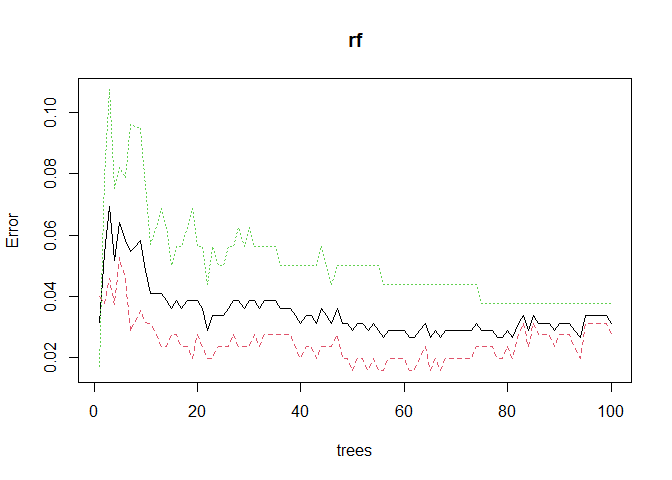
\includegraphics{C:/Users/nilve/Documents/GitHub/diabetes-data-diving/notebooks/random_forest_files/figure-gfm/error-1.png}
\caption{}
\end{figure}

\hypertarget{header-n967}{%
\subsubsection{Variable Importance}\label{header-n967}}

\begin{Shaded}
\begin{Highlighting}[]
\KeywordTok{par}\NormalTok{(}\DataTypeTok{bg=}\StringTok{"#f2f2f2"}\NormalTok{)}
\KeywordTok{varImpPlot}\NormalTok{(rf, }\DataTypeTok{main=}\StringTok{"Variable Importance Plot"}\NormalTok{, }\DataTypeTok{type=}\DecValTok{1}\NormalTok{, }\DataTypeTok{pch=}\DecValTok{19}\NormalTok{)}
\end{Highlighting}
\end{Shaded}

\begin{figure}
\centering
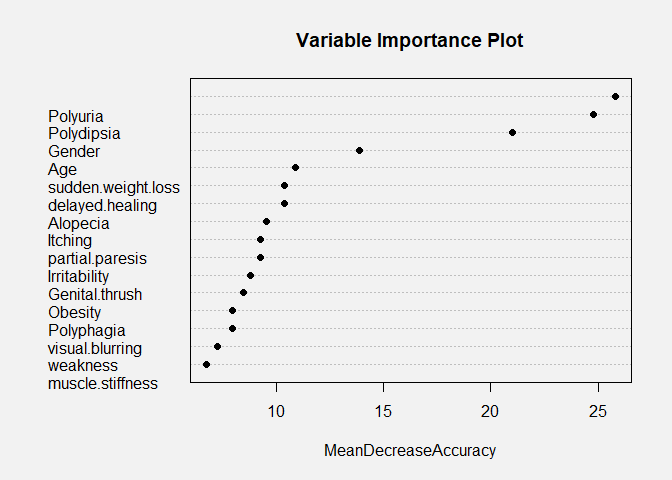
\includegraphics{C:/Users/nilve/Documents/GitHub/diabetes-data-diving/notebooks/random_forest_files/figure-gfm/var-1.png}
\caption{}
\end{figure}

The random forest model is very interesting because it can allow us to
investigate the relative importance of the variables that we use in our
model. In the variable importance plot above, we see that polydipsia,
polyuria, gender, and age are the four most important variables in our
model. This is determined by computing the
\texttt{MeanDecreaseAccuracy}. This quantity is calculated by changing
the values in each feature and then observing how much that change
decreases the accuracy of the model. An interesting conclusion from this
plot is that age is very important to the accuracy of the model. In our
density plots above, we concluded that there was only a slight
difference in the mean ages between the patients that had diabetes and
did not have diabetes, and age also was not statistically significant in
the linear model. Therefore, it is likely that age has a nonlinear
relationship with the diabetes status of a patient or that age in
combination with another factor is an important predictor.

\hypertarget{header-n971}{%
\subsubsection{Validating on the Testing Set}\label{header-n971}}

Seeing that the model had good accuracy on the training set and the
conclusions from the variable importance plot are reasonable, we can now
validate our model on the remaining 20\% of the dataset. We use our
random forest model to generate predictions for the remaining samples
and then compare those with the observed diabetes status of those
patients. Finally, we can visualize this with a confusion matrix.

\begin{Shaded}
\begin{Highlighting}[]
\NormalTok{prediction_for_table <-}\StringTok{ }\KeywordTok{predict}\NormalTok{(rf,test[,}\OperatorTok{-}\DecValTok{17}\NormalTok{])}
\NormalTok{confusion <-}\StringTok{ }\KeywordTok{table}\NormalTok{(}\DataTypeTok{observed=}\NormalTok{test[[}\DecValTok{17}\NormalTok{]],}\DataTypeTok{predicted=}\NormalTok{prediction_for_table)}
\NormalTok{confusion}
\end{Highlighting}
\end{Shaded}

\begin{verbatim}
##           predicted
## observed   Positive Negative
##   Positive       64        0
##   Negative        2       38
\end{verbatim}

\begin{Shaded}
\begin{Highlighting}[]
\NormalTok{true_class <-}\StringTok{ }\KeywordTok{factor}\NormalTok{(}\KeywordTok{c}\NormalTok{(}\StringTok{'Negative'}\NormalTok{, }\StringTok{'Negative'}\NormalTok{, }\StringTok{'Positive'}\NormalTok{, }\StringTok{'Positive'}\NormalTok{))}
\NormalTok{predicted_class <-}\StringTok{ }\KeywordTok{factor}\NormalTok{(}\KeywordTok{c}\NormalTok{(}\StringTok{'Negative'}\NormalTok{, }\StringTok{'Positive'}\NormalTok{, }\StringTok{'Negative'}\NormalTok{, }\StringTok{'Positive'}\NormalTok{))}
\NormalTok{counts      <-}\StringTok{ }\KeywordTok{c}\NormalTok{(confusion[}\DecValTok{2}\NormalTok{,}\DecValTok{2}\NormalTok{], confusion[}\DecValTok{2}\NormalTok{,}\DecValTok{1}\NormalTok{], confusion[}\DecValTok{1}\NormalTok{,}\DecValTok{2}\NormalTok{], confusion[}\DecValTok{1}\NormalTok{,}\DecValTok{1}\NormalTok{])}
\NormalTok{df <-}\StringTok{ }\KeywordTok{data.frame}\NormalTok{(true_class, predicted_class, counts)}


\KeywordTok{ggplot}\NormalTok{(}\DataTypeTok{data =}\NormalTok{  df, }\DataTypeTok{mapping =} \KeywordTok{aes}\NormalTok{(}\DataTypeTok{x =}\NormalTok{ true_class, }\DataTypeTok{y =}\NormalTok{ predicted_class)) }\OperatorTok{+}
\StringTok{  }\KeywordTok{geom_tile}\NormalTok{(}\KeywordTok{aes}\NormalTok{(}\DataTypeTok{fill =}\NormalTok{ counts), }\DataTypeTok{colour =} \StringTok{"white"}\NormalTok{) }\OperatorTok{+}
\StringTok{  }\KeywordTok{geom_text}\NormalTok{(}\KeywordTok{aes}\NormalTok{(}\DataTypeTok{label =} \KeywordTok{sprintf}\NormalTok{(}\StringTok{"%1.0f"}\NormalTok{, counts)), }\DataTypeTok{vjust =} \DecValTok{1}\NormalTok{, }\DataTypeTok{colour=}\StringTok{"white"}\NormalTok{) }\OperatorTok{+}
\StringTok{  }\KeywordTok{scale_fill_gradient}\NormalTok{() }\OperatorTok{+}
\StringTok{  }\KeywordTok{theme_bw}\NormalTok{() }\OperatorTok{+}\StringTok{ }\KeywordTok{theme}\NormalTok{(}\DataTypeTok{legend.position =} \StringTok{"none"}\NormalTok{) }\OperatorTok{+}
\StringTok{  }\KeywordTok{labs}\NormalTok{(}\DataTypeTok{title=}\StringTok{"Confusion Matrix"}\NormalTok{,}\DataTypeTok{x=}\StringTok{"True Class"}\NormalTok{, }\DataTypeTok{y=}\StringTok{"Predicted Class"}\NormalTok{)}\OperatorTok{+}
\StringTok{  }\KeywordTok{theme}\NormalTok{(}\DataTypeTok{plot.title =} \KeywordTok{element_text}\NormalTok{(}\DataTypeTok{hjust =} \FloatTok{0.5}\NormalTok{)) }\OperatorTok{+}
\StringTok{  }\KeywordTok{theme}\NormalTok{(}\DataTypeTok{plot.background =} \KeywordTok{element_rect}\NormalTok{(}\DataTypeTok{fill =} \StringTok{'#f2f2f2'}\NormalTok{, }\DataTypeTok{colour =} \StringTok{'#f2f2f2'}\NormalTok{)) }\OperatorTok{+}
\StringTok{  }\KeywordTok{theme}\NormalTok{(}\DataTypeTok{panel.background =} \KeywordTok{element_rect}\NormalTok{(}\DataTypeTok{fill =} \StringTok{'#f2f2f2'}\NormalTok{, }\DataTypeTok{colour =} \StringTok{'#f2f2f2'}\NormalTok{))}
\end{Highlighting}
\end{Shaded}

\begin{figure}
\centering
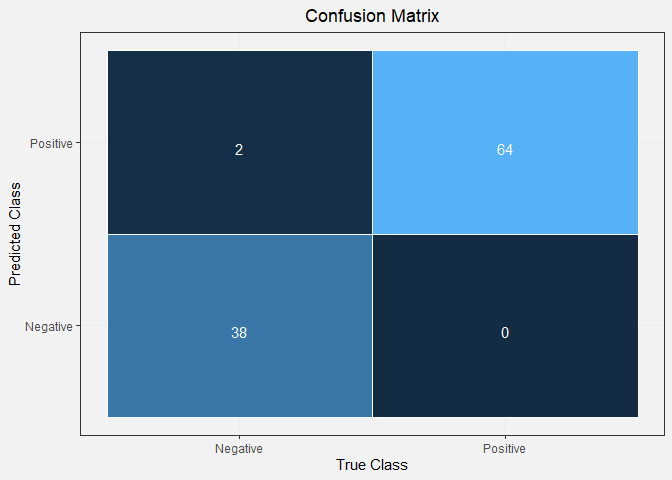
\includegraphics{C:/Users/nilve/Documents/GitHub/diabetes-data-diving/notebooks/random_forest_files/figure-gfm/confusion-1.png}
\caption{}
\end{figure}

\begin{Shaded}
\begin{Highlighting}[]
\NormalTok{test_accuracy <-}\StringTok{ }\NormalTok{(confusion[}\DecValTok{2}\NormalTok{,}\DecValTok{2}\NormalTok{] }\OperatorTok{+}\StringTok{ }\NormalTok{confusion[}\DecValTok{1}\NormalTok{,}\DecValTok{1}\NormalTok{])}\OperatorTok{/}\KeywordTok{sum}\NormalTok{(confusion)}
\KeywordTok{print}\NormalTok{(test_accuracy)}
\end{Highlighting}
\end{Shaded}

\begin{verbatim}
## [1] 0.9807692
\end{verbatim}

From our confusion matrix, we can see that the testing accuracy of our
model is 98.1\%. This value is similar to that of our training accuracy,
indicating that our model is not over-fitting to the data. These model
accuracy values are very good, and our model has great predictive power.
We can do further hyper-parameter tuning to improve our model more, but
that is out of the scope of this project.

\hypertarget{header-n982}{%
\section{Conclusion}\label{header-n982}}

Overall, the presence of conditions such as polyuria, polydipsia, sudden
weight loss, and partial paresis increased the likelihood that a patient
has diabetes. The random forest model showed to be a very accurate model
for predicting diabetes unlike the linear model. Therefore, the random
forest model indicates the polyuria, polydipsia, age, and gender are the
useful features for predicting the diagnosis of diabetes.

\end{document}
